\documentclass[aspectratio=169, 10pt]{beamer}

% ---------- Tema y colores ----------
\usetheme{default}
\usecolortheme{default}
\setbeamertemplate{navigation symbols}{}
\setbeamertemplate{footline}[frame number]
\setbeamertemplate{frametitle continuation}{}

\definecolor{StanfordRed}{RGB}{140,21,21}
\definecolor{LightGray}{RGB}{240,240,240}
\definecolor{AccentGreen}{RGB}{0,130,100}
\definecolor{UCMBlue}{RGB}{4, 171, 226}
\definecolor{UCMNavy}{RGB}{20, 65, 134}

\definecolor{mitblue}{RGB}{20, 65, 134}
\definecolor{mitgray}{RGB}{169, 169, 169}

\setbeamercolor{frametitle}{fg=white, bg=UCMBlue}
\setbeamercolor{title}{fg=white}
\setbeamercolor{author}{fg=white}
\setbeamercolor{institute}{fg=white!80}
\setbeamercolor{structure}{fg=UCMBlue}
\setbeamercolor{block title}{bg=UCMBlue!15!white, fg=UCMBlue}
\setbeamercolor{block body}{bg=LightGray}
\setbeamercolor{block title alerted}{bg=StanfordRed!15!white, fg=StanfordRed}
\setbeamercolor{block body alerted}{bg=LightGray}
\setbeamercolor{alerted text}{fg=UCMBlue}

\setbeamerfont{frametitle}{series=\bfseries, size=\large}
\setbeamerfont{title}{series=\bfseries, size=\LARGE}
\setbeamerfont{block title}{series=\bfseries}

% ---------- Paquetes ----------
\usepackage[utf8]{inputenc}
\usepackage[T1]{fontenc}
\usepackage[provide=*,spanish]{babel}
\usepackage{amsmath, amssymb}
\usepackage{graphicx}
\usepackage{tikz}
\usepackage{pgfplots}
\pgfplotsset{compat=1.18}
\usetikzlibrary{arrows, arrows.meta, shapes, shapes.geometric, positioning,
	fit, calc, matrix, chains, decorations.pathreplacing,
	backgrounds, shadows}
\usepackage{booktabs}
\usepackage{array}
\usepackage{xcolor}
\usepackage{multicol}
\usepackage{tcolorbox}
\tcbuselibrary{skins, breakable}
\usepackage{fontawesome5}

% ---------- Comandos \'utiles ----------
\providecommand{\R}{\mathbb{R}}
\newcommand{\V}{\mathcal{V}}
\newcommand{\tok}[1]{\texttt{#1}}
\newcommand{\good}{{\color{AccentGreen}\faCheck}}
\newcommand{\bad}{{\color{StanfordRed}\faTimes}}

\newcommand{\formula}[1]{%
	\begin{tcolorbox}[colback=UCMBlue!8, colframe=UCMBlue, arc=4pt,
		boxsep=2pt, left=6pt, right=6pt, top=3pt, bottom=3pt]
		#1
	\end{tcolorbox}
}

\tcbset{codebox/.style={colback=LightGray, colframe=UCMNavy, arc=3pt, boxsep=1pt, left=4pt, right=4pt, top=2pt, bottom=2pt}}

% ---------- Portada ----------
\title{\textbf{Introducci\'on al Procesamiento de Lenguaje Natural}}
\subtitle{Conceptos, metodolog\'ias y ciclo de vida de los datos}
\author{Sergio Hern\'andez, PhD\\ shernandez@ucm.cl}
\institute{
	\begin{tikzpicture}[scale=0.42, every node/.style={transform shape}]
		\foreach \i/\y in {1/0,2/1,3/2}{\node[circle,draw=white,fill=white!20,minimum size=4mm] (i\i) at (0,\y){};}
		\foreach \i/\y in {1/-0.5,2/0.5,3/1.5,4/2.5}{\node[circle,draw=white,fill=white!35,minimum size=4mm] (h\i) at (2,\y){};}
		\foreach \i/\y in {1/0.5,2/1.5}{\node[circle,draw=white,fill=white!50,minimum size=4mm] (o\i) at (4,\y){};}
		\foreach \a in {1,2,3}\foreach \b in {1,2,3,4}{\draw[white,opacity=0.5] (i\a)--(h\b);}
		\foreach \a in {1,2,3,4}\foreach \b in {1,2}{\draw[white,opacity=0.5] (h\a)--(o\b);}
	\end{tikzpicture}
	\\ \textbf{Mag\'ister en Data Science --- Universidad Cat\'olica del Maule}}
\date{}

\begin{document}
% --- T\'itulo ---
{
	\setbeamertemplate{background}{
		\begin{tikzpicture}[remember picture, overlay]
			\fill[UCMBlue] (current page.south west) rectangle (current page.north east);
			\fill[UCMBlue!70!black, opacity=0.5]
			(current page.south west) -- ++(0,3) -- ++(18,0) -- cycle;
			\foreach \i in {1,...,40}{
				\fill[white, opacity=0.04]
				({random()*17}, {random()*10}) circle ({random()*0.3});
			}
		\end{tikzpicture}
	}
	\begin{frame}[plain]
		\vspace{1.2cm}
		\titlepage
		\begin{tikzpicture}[remember picture, overlay]
			\node[white, opacity=0.15, font=\fontsize{80}{80}\selectfont]
			at (current page.east) [xshift=-2.4cm] {$\mathbf{v}_w$};
		\end{tikzpicture}
	\end{frame}
}

% =================================================================
\section{Introducci\'on}

\begin{frame}{¿Qu\'e es el Procesamiento de Lenguaje Natural?}

	\begin{columns}[T]
		\begin{column}{0.55\textwidth}
			\begin{block}{Definici\'on}
				El \textbf{Procesamiento de Lenguaje Natural} (NLP) estudia la interacci\'on entre computadores y personas mediante \textbf{lenguajes naturales}: espa\~nol, ingl\'es, mapudungun\ldots
			\end{block}

			\vspace{0.2cm}

			\begin{itemize}
				\item Los humanos generamos enormes vol\'umenes de texto: noticias, redes sociales, fichas cl\'inicas, contratos, c\'odigo.
				\item El objetivo es \textbf{comprender} y \textbf{generar} texto de forma \'util.
				\item En la pr\'actica: convertir texto en \textbf{tensores} que una red neuronal pueda procesar.
			\end{itemize}
		\end{column}

		\begin{column}{0.42\textwidth}
			\begin{block}{¿Por qu\'e es dif\'icil?}
				\small
				\begin{itemize}
					\item \textbf{Discreto}: palabras, no p\'ixeles; no hay noci\'on natural de distancia.
					\item \textbf{Ambiguo}: ``fui al \textit{banco} a depositar'' vs.\ ``me sent\'e en el \textit{banco}''.
					\item \textbf{Secuencial y de largo alcance}: el orden importa y las dependencias pueden estar lejos.
					\item \textbf{Ley de Zipf}: pocas palabras muy frecuentes, una cola larga de palabras raras.
					\item \textbf{Composicional}: ``hot dog'' $\neq$ ``hot'' $+$ ``dog''.
				\end{itemize}
			\end{block}
		\end{column}
	\end{columns}

\end{frame}

\begin{frame}{Tareas T\'ipicas de NLP}

	\begin{columns}[T]
		\begin{column}{0.5\textwidth}
			\begin{block}{Nivel de secuencia}
				\small
				\begin{itemize}
					\item \textbf{Clasificaci\'on de texto}: t\'opico de una noticia, an\'alisis de sentimiento, detecci\'on de spam.
					\item \textbf{Pares de textos}: inferencia en lenguaje natural (NLI), similitud sem\'antica, detecci\'on de par\'afrasis.
				\end{itemize}
			\end{block}

			\begin{block}{Nivel de token}
				\small
				\begin{itemize}
					\item \textbf{Etiquetado de secuencias}: etiquetas gramaticales (POS), reconocimiento de entidades (NER).
					\item \textbf{Respuesta a preguntas extractiva}: marcar el inicio y fin de la respuesta en un texto.
				\end{itemize}
			\end{block}
		\end{column}

		\begin{column}{0.5\textwidth}
			\begin{block}{Generaci\'on (secuencia a secuencia)}
				\small
				\begin{itemize}
					\item Traducci\'on autom\'atica.
					\item Resumen de documentos.
					\item Di\'alogo y asistentes (LLMs).
				\end{itemize}
			\end{block}

			\vspace{0.2cm}

			\begin{alertblock}{En esta clase}
				\small
				Usamos \textbf{clasificaci\'on de noticias} (AG\_NEWS) como tarea gu\'ia: 4 clases \emph{World, Sports, Business, Sci/Tech}. Es la tarea del laboratorio 3.1.
			\end{alertblock}
		\end{column}
	\end{columns}

\end{frame}

\begin{frame}{Evoluci\'on de los M\'etodos de NLP}

	\centering
	\resizebox{\textwidth}{!}{%
	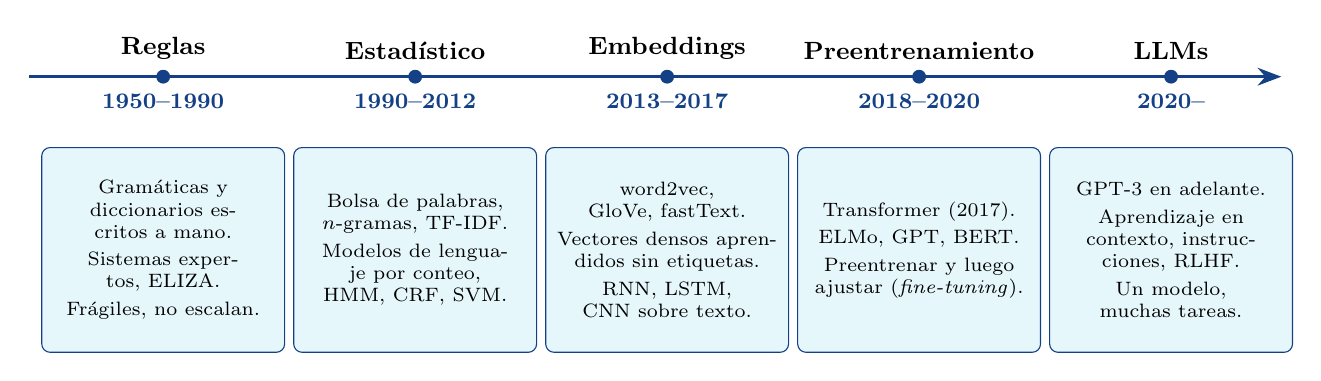
\begin{tikzpicture}[
			era/.style={draw=UCMNavy, fill=UCMBlue!10, rounded corners=3pt, text width=2.85cm, align=center, minimum height=2.6cm, font=\scriptsize},
			yr/.style={font=\footnotesize\bfseries, text=UCMNavy}
		]
		\draw[-{Stealth[length=3mm]}, line width=1.2pt, UCMNavy] (-0.3,0) -- (15.6,0);
		\foreach \x/\y/\t in {1.4/1950--1990/Reglas, 4.6/1990--2012/Estad\'istico, 7.8/2013--2017/Embeddings, 11.0/2018--2020/Preentrenamiento, 14.2/2020--/LLMs}{
			\fill[UCMNavy] (\x,0) circle (2.5pt);
			\node[yr, below] at (\x,-0.1) {\y};
			\node[font=\small\bfseries, above] at (\x,0.1) {\t};
		}
		\node[era] at (1.4,-2.2) {Gram\'aticas y diccionarios escritos a mano.\\[2pt] Sistemas expertos, ELIZA.\\[2pt] Fr\'agiles, no escalan.};
		\node[era] at (4.6,-2.2) {Bolsa de palabras, $n$-gramas, TF-IDF.\\[2pt] Modelos de lenguaje por conteo, HMM, CRF, SVM.};
		\node[era] at (7.8,-2.2) {word2vec, GloVe, fastText.\\[2pt] Vectores densos aprendidos sin etiquetas.\\[2pt] RNN, LSTM, CNN sobre texto.};
		\node[era] at (11.0,-2.2) {Transformer (2017).\\[2pt] ELMo, GPT, BERT.\\[2pt] Preentrenar y luego ajustar (\textit{fine-tuning}).};
		\node[era] at (14.2,-2.2) {GPT-3 en adelante.\\[2pt] Aprendizaje en contexto, instrucciones, RLHF.\\[2pt] Un modelo, muchas tareas.};
	\end{tikzpicture}}

	\vspace{0.3cm}

	\small
	Hilo conductor: cada etapa \textbf{reduce el trabajo manual} de dise\~no de caracter\'isticas y \textbf{aumenta la cantidad de datos} que se aprovecha.

\end{frame}

% =================================================================
\section{Metodolog\'ias}

\begin{frame}{El Paradigma Actual: Preentrenar y Ajustar}

	\centering
	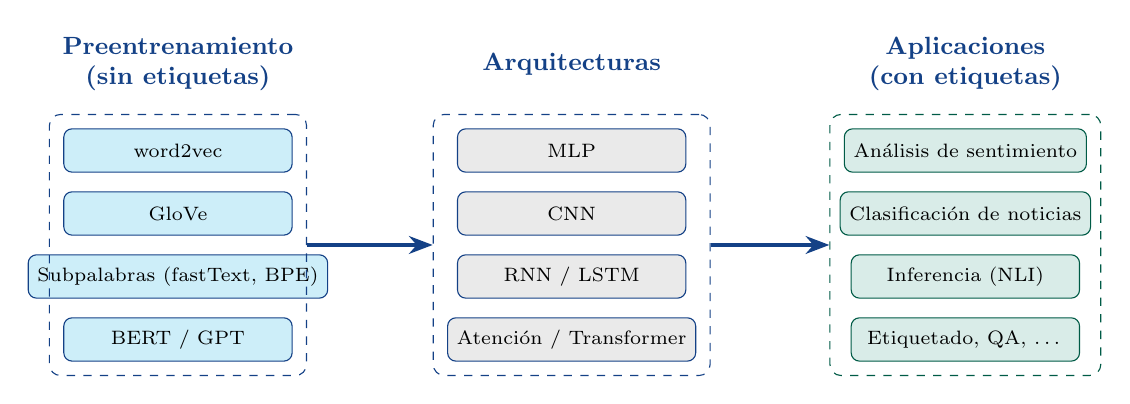
\begin{tikzpicture}[
			box/.style={draw=UCMNavy, rounded corners=3pt, minimum width=2.9cm, minimum height=0.55cm, font=\scriptsize, align=center},
			pre/.style={box, fill=UCMBlue!20},
			arc/.style={box, fill=mitgray!25},
			app/.style={box, fill=AccentGreen!15, draw=AccentGreen!70!black},
			hdr/.style={font=\small\bfseries, text=UCMNavy, align=center}
		]
		\node[hdr] at (0,2.3) {Preentrenamiento\\(sin etiquetas)};
		\node[hdr] at (5,2.3) {Arquitecturas};
		\node[hdr] at (10,2.3) {Aplicaciones\\(con etiquetas)};

		\node[pre] (p1) at (0,1.2) {word2vec};
		\node[pre] (p2) at (0,0.4) {GloVe};
		\node[pre] (p3) at (0,-0.4) {Subpalabras (fastText, BPE)};
		\node[pre] (p4) at (0,-1.2) {BERT / GPT};

		\node[arc] (a1) at (5,1.2) {MLP};
		\node[arc] (a2) at (5,0.4) {CNN};
		\node[arc] (a3) at (5,-0.4) {RNN / LSTM};
		\node[arc] (a4) at (5,-1.2) {Atenci\'on / Transformer};

		\node[app] (s1) at (10,1.2) {An\'alisis de sentimiento};
		\node[app] (s2) at (10,0.4) {Clasificaci\'on de noticias};
		\node[app] (s3) at (10,-0.4) {Inferencia (NLI)};
		\node[app] (s4) at (10,-1.2) {Etiquetado, QA, \ldots};

		\node[draw=UCMNavy, dashed, rounded corners, fit=(p1)(p4), inner sep=5pt] (P) {};
		\node[draw=UCMNavy, dashed, rounded corners, fit=(a1)(a4), inner sep=5pt] (A) {};
		\node[draw=AccentGreen!70!black, dashed, rounded corners, fit=(s1)(s4), inner sep=5pt] (S) {};
		\draw[-{Stealth[length=3mm]}, line width=1.5pt, UCMNavy] (P.east) -- (A.west);
		\draw[-{Stealth[length=3mm]}, line width=1.5pt, UCMNavy] (A.east) -- (S.west);
	\end{tikzpicture}

	\vspace{0.3cm}

	\begin{itemize}
		\small
		\item \textbf{Aguas arriba}: aprender representaciones de texto a partir de corpus masivos \emph{sin etiquetar}.
		\item \textbf{Aguas abajo}: reutilizarlas en una arquitectura para una tarea concreta con \emph{pocos} datos etiquetados.
	\end{itemize}

	\vspace{-0.1cm}
	{\tiny Adaptado de Zhang et al., \textit{Dive into Deep Learning}, Fig.\ 15.1.}

\end{frame}

\begin{frame}{Aprendizaje Autosupervisado}

	\begin{columns}[T]
		\begin{column}{0.52\textwidth}
			\begin{block}{Idea}
				Ocultar una parte del texto y \textbf{predecirla a partir del resto}. El propio texto entrega la supervisi\'on: no hay costo de etiquetado.
			\end{block}

			\vspace{0.2cm}

			\begin{itemize}
				\small
				\item word2vec: predecir palabras vecinas de una palabra central.
				\item GloVe: reproducir las co-ocurrencias globales del corpus.
				\item BERT: predecir palabras enmascaradas usando ambos lados.
				\item GPT: predecir la \emph{siguiente} palabra.
			\end{itemize}
		\end{column}

		\begin{column}{0.45\textwidth}
			\centering
			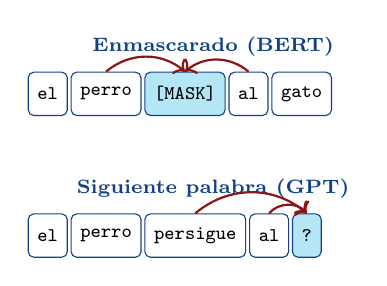
\begin{tikzpicture}[
					w/.style={draw=UCMNavy, rounded corners=2pt, minimum height=0.55cm, font=\scriptsize\ttfamily, fill=white},
					m/.style={w, fill=UCMBlue!30, font=\scriptsize\bfseries\ttfamily}
				]
				\node[font=\scriptsize\bfseries, text=UCMNavy] at (2.1,1.9) {Enmascarado (BERT)};
				\node[w] (a1) at (0,1.3) {el};
				\node[w, right=1pt of a1] (a2) {perro};
				\node[m, right=1pt of a2] (a3) {[MASK]};
				\node[w, right=1pt of a3] (a4) {al};
				\node[w, right=1pt of a4] (a5) {gato};
				\draw[->, StanfordRed, thick] (a2.north) to[bend left=40] (a3.north);
				\draw[->, StanfordRed, thick] (a4.north) to[bend right=40] (a3.north);

				\node[font=\scriptsize\bfseries, text=UCMNavy] at (2.1,0.1) {Siguiente palabra (GPT)};
				\node[w] (b1) at (0,-0.5) {el};
				\node[w, right=1pt of b1] (b2) {perro};
				\node[w, right=1pt of b2] (b3) {persigue};
				\node[w, right=1pt of b3] (b4) {al};
				\node[m, right=1pt of b4] (b5) {?};
				\draw[->, StanfordRed, thick] (b4.north) to[bend left=50] (b5.north);
				\draw[->, StanfordRed, thick] (b3.north) to[bend left=40] (b5.north);
			\end{tikzpicture}

			\vspace{0.3cm}

			\begin{alertblock}{Consecuencia}
				\small
				Se pueden usar miles de millones de palabras (Wikipedia, libros, la web) para aprender qu\'e \emph{significa} cada palabra.
			\end{alertblock}
		\end{column}
	\end{columns}

\end{frame}

\begin{frame}{Metodolog\'ias de Representaci\'on: Un Mapa}

	\begin{center}
		\footnotesize
		\begin{tabular}{@{}llll@{}}
			\toprule
			\textbf{Familia} & \textbf{Ejemplos} & \textbf{Vector por} & \textbf{Captura} \\
			\midrule
			Dispersa, por conteo & One-hot, BoW, TF-IDF, $n$-gramas & documento & frecuencia, palabras clave \\
			Densa, est\'atica & word2vec, GloVe & palabra & similitud sem\'antica \\
			Densa, subpalabra & fastText, BPE & fragmento de palabra & morfolog\'ia, palabras raras \\
			Densa, contextual & ELMo, BERT, GPT & token \emph{en su contexto} & polisemia, sintaxis \\
			\bottomrule
		\end{tabular}
	\end{center}

	\vspace{0.3cm}

	\begin{columns}[T]
		\begin{column}{0.48\textwidth}
			\begin{block}{Dispersa}
				\small
				Dimensi\'on $= |\V|$ (decenas de miles a millones). Interpretable, barata, sin noci\'on de significado.
			\end{block}
		\end{column}
		\begin{column}{0.48\textwidth}
			\begin{block}{Densa}
				\small
				Dimensi\'on $d \approx 50$--$1024$. Aprendida; palabras parecidas $\Rightarrow$ vectores cercanos.
			\end{block}
		\end{column}
	\end{columns}

\end{frame}

% =================================================================
\section{Ciclo de Vida de los Datos}

\begin{frame}{Ciclo de Vida de los Datos en NLP}

	\begin{columns}[c]
		\begin{column}{0.55\textwidth}
			\centering
			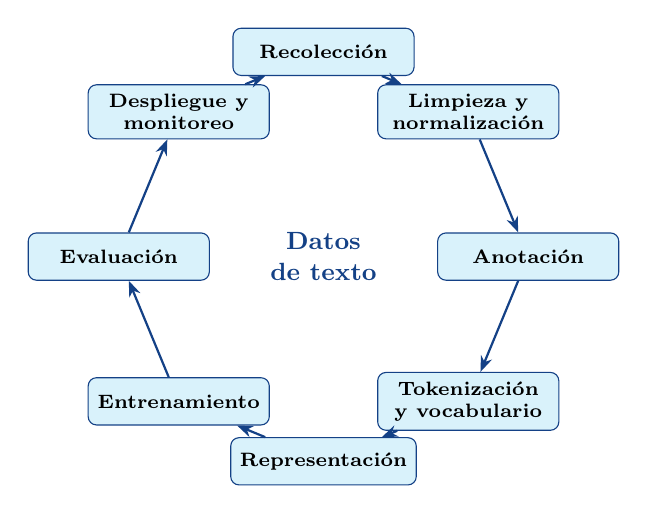
\begin{tikzpicture}[
					st/.style={draw=UCMNavy, fill=UCMBlue!15, rounded corners=3pt, minimum width=2.3cm, minimum height=0.6cm, font=\scriptsize\bfseries, align=center}
				]
				\foreach \a/\t/\n in {90/Recolecci\'on/s1, 45/Limpieza y\\normalizaci\'on/s2, 0/Anotaci\'on/s3, -45/Tokenizaci\'on\\y vocabulario/s4, -90/Representaci\'on/s5, -135/Entrenamiento/s6, 180/Evaluaci\'on/s7, 135/Despliegue y\\monitoreo/s8}{
					\node[st] (\n) at (\a:2.6) {\t};
				}
				\foreach \i/\j in {s1/s2, s2/s3, s3/s4, s4/s5, s5/s6, s6/s7, s7/s8, s8/s1}{
					\draw[-{Stealth[length=2mm]}, UCMNavy, thick] (\i) -- (\j);
				}
				\node[font=\small\bfseries, text=UCMNavy, align=center] at (0,0) {Datos\\de texto};
			\end{tikzpicture}
		\end{column}

		\begin{column}{0.43\textwidth}
			\begin{itemize}
				\small
				\item Es un \textbf{ciclo}: el monitoreo en producci\'on revela nuevos datos que recolectar y errores que anotar.
				\item En NLP, la mayor parte del esfuerzo est\'a \textbf{antes} del modelo: fuentes, limpieza, etiquetas y tokenizaci\'on.
				\item Decisiones tempranas (p.\ ej.\ pasar a min\'usculas, tama\~no del vocabulario) \textbf{limitan} lo que el modelo puede aprender.
			\end{itemize}

			\vspace{0.2cm}

			\begin{alertblock}{Regla pr\'actica}
				\small
				Un modelo es tan bueno como el corpus con que se entren\'o y tan confiable como el conjunto con que se evalu\'o.
			\end{alertblock}
		\end{column}
	\end{columns}

\end{frame}

\begin{frame}{1. Recolecci\'on: Corpus y Fuentes}

	\begin{columns}[T]
		\begin{column}{0.5\textwidth}
			\begin{block}{Corpus usados en esta unidad}
				\scriptsize
				\begin{tabular}{@{}lp{3.6cm}@{}}
					\toprule
					\textbf{Corpus} & \textbf{Contenido} \\
					\midrule
					AG\_NEWS & 120\,000 / 7\,600 titulares (train/test), 4 clases \\
					Penn Treebank (PTB) & Wall Street Journal; 42\,069 oraciones de entrenamiento \\
					WikiText-2 & Art\'iculos de Wikipedia; conserva may\'usculas, puntuaci\'on y n\'umeros \\
					BookCorpus & $\sim$800 M palabras (libros) \\
					Wikipedia (ingl\'es) & $\sim$2\,500 M palabras \\
					\bottomrule
				\end{tabular}
			\end{block}
		\end{column}

		\begin{column}{0.47\textwidth}
			\begin{block}{Preguntas antes de recolectar}
				\small
				\begin{itemize}
					\item \textbf{Representatividad}: ¿el dominio, idioma y registro coinciden con el uso real?
					\item \textbf{Licencia y privacidad}: derechos de autor, datos personales, fichas cl\'inicas.
					\item \textbf{Sesgos}: estereotipos presentes en el texto pasan a los vectores.
					\item \textbf{Calidad}: duplicados, spam, texto generado autom\'aticamente.
				\end{itemize}
			\end{block}
		\end{column}
	\end{columns}

\end{frame}

\begin{frame}{2. Limpieza y Normalizaci\'on}

	\begin{columns}[T]
		\begin{column}{0.5\textwidth}
			\begin{block}{Operaciones habituales}
				\small
				\begin{itemize}
					\item Pasar a \textbf{min\'usculas}.
					\item Separar la \textbf{puntuaci\'on} del token anterior.
					\item Eliminar marcado (HTML), normalizar Unicode, tildes y espacios.
					\item Reemplazar palabras raras por \tok{<unk>}.
					\item Segmentar en oraciones y p\'arrafos.
				\end{itemize}
			\end{block}

			\vspace{0.1cm}
			{\small Cada decisi\'on \textbf{pierde informaci\'on}: en min\'usculas, ``Apple'' (empresa) y ``apple'' (fruta) se funden.}
		\end{column}

		\begin{column}{0.47\textwidth}
			\begin{block}{Ejemplo: preparaci\'on de WikiText-2 (d2l)}
				\small
				\begin{enumerate}
					\item Cada l\'inea es un p\'arrafo.
					\item Insertar espacio antes de la puntuaci\'on.
					\item Conservar s\'olo p\'arrafos con $\geq 2$ oraciones.
					\item Separar oraciones por ``\tok{ . }''.
					\item Pasar a min\'usculas y barajar p\'arrafos.
				\end{enumerate}
			\end{block}

			\begin{block}{Ejemplo: AG\_NEWS}
				\scriptsize
				\texttt{"Wall St.\ Bears Claw Back Into the Black (Reuters) Reuters - Short-sellers, Wall Street's dwindling\textbackslash band of ultra-cynics\ldots"}\\[2pt]
				Contiene saltos de l\'inea escapados (\texttt{\textbackslash}) y la fuente repetida.
			\end{block}
		\end{column}
	\end{columns}

\end{frame}

\begin{frame}{3. Anotaci\'on y Particiones}

	\begin{columns}[T]
		\begin{column}{0.5\textwidth}
			\begin{block}{Anotaci\'on}
				\small
				\begin{itemize}
					\item Gu\'ia de anotaci\'on con definiciones y ejemplos l\'imite.
					\item Varios anotadores por ejemplo; medir el \textbf{acuerdo inter-anotador} (kappa de Cohen):
				\end{itemize}
				\formula{\centering $\kappa = \dfrac{p_o - p_e}{1 - p_e}$}
				\scriptsize $p_o$: acuerdo observado; $p_e$: acuerdo esperado por azar.
			\end{block}

			{\small El preentrenamiento autosupervisado \emph{evita} este paso: las etiquetas salen del propio texto.}
		\end{column}

		\begin{column}{0.47\textwidth}
			\begin{block}{Particiones}
				\small
				\begin{itemize}
					\item Entrenamiento / validaci\'on / prueba, \textbf{estratificadas} por clase.
					\item El \textbf{vocabulario} y las estad\'isticas (IDF, frecuencias) se calculan s\'olo con entrenamiento.
				\end{itemize}
			\end{block}

			\begin{alertblock}{Fugas de datos t\'ipicas en texto}
				\small
				\begin{itemize}
					\item Duplicados o casi duplicados entre train y test.
					\item El mismo autor o documento repartido entre particiones.
					\item Corpus de preentrenamiento que contiene el conjunto de prueba (\emph{contaminaci\'on}).
				\end{itemize}
			\end{alertblock}
		\end{column}
	\end{columns}

\end{frame}

\begin{frame}{4. Evaluaci\'on, Despliegue y Monitoreo}

	\begin{columns}[T]
		\begin{column}{0.5\textwidth}
			\begin{block}{M\'etricas}
				\small
				\begin{itemize}
					\item \textbf{Clasificaci\'on}: exactitud; con clases desbalanceadas, precisi\'on, \textit{recall} y $F_1$ macro.
					\item \textbf{Modelos de lenguaje}: perplejidad
				\end{itemize}
				\formula{\centering $\mathrm{PPL} = \exp\Big(-\dfrac{1}{T}\displaystyle\sum_{t=1}^{T} \log P(w_t \mid w_{<t})\Big)$}
				\begin{itemize}
					\small
					\item \textbf{Embeddings}: similitud y analog\'ias (evaluaci\'on intr\'inseca) o desempe\~no en la tarea final (extr\'inseca).
				\end{itemize}
			\end{block}
		\end{column}

		\begin{column}{0.47\textwidth}
			\begin{block}{En producci\'on}
				\small
				\begin{itemize}
					\item \textbf{Deriva de datos}: aparecen palabras, temas y estilos nuevos (el vocabulario de 2019 no conoc\'ia ``COVID'').
					\item Tasa de \tok{<unk>} como indicador temprano.
					\item Reentrenar con datos nuevos anotados: el ciclo se cierra.
				\end{itemize}
			\end{block}

			\begin{block}{Documentaci\'on}
				\small
				\textit{Datasheets for Datasets} y \textit{Data/Model Cards}: origen, composici\'on, usos previstos y limitaciones del corpus y del modelo.
			\end{block}
		\end{column}
	\end{columns}

\end{frame}

% =================================================================
\section{Del Texto a Tensores}

\begin{frame}{Tokenizaci\'on y Vocabulario}

	\centering
	\resizebox{\textwidth}{!}{%
	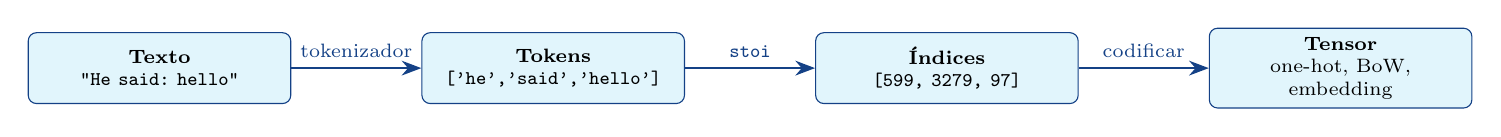
\begin{tikzpicture}[
			st/.style={draw=UCMNavy, fill=UCMBlue!12, rounded corners=3pt, minimum height=0.9cm, text width=3.1cm, align=center, font=\scriptsize},
			arr/.style={-{Stealth[length=2.5mm]}, thick, UCMNavy}
		]
		\node[st] (t) at (0,0) {\textbf{Texto}\\\texttt{"He said: hello"}};
		\node[st] (k) at (5.0,0) {\textbf{Tokens}\\\texttt{['he','said','hello']}};
		\node[st] (i) at (10.0,0) {\textbf{\'Indices}\\\texttt{[599, 3279, 97]}};
		\node[st] (v) at (15.0,0) {\textbf{Tensor}\\one-hot, BoW, embedding};
		\draw[arr] (t) -- node[above, font=\scriptsize] {tokenizador} (k);
		\draw[arr] (k) -- node[above, font=\scriptsize] {\texttt{stoi}} (i);
		\draw[arr] (i) -- node[above, font=\scriptsize] {codificar} (v);
	\end{tikzpicture}}

	\vspace{0.3cm}

	\begin{columns}[T]
		\begin{column}{0.48\textwidth}
			\begin{block}{Token}
				\small
				Unidad m\'inima que procesa el modelo: \textbf{palabra}, \textbf{car\'acter} o \textbf{subpalabra}. Es un compromiso:
				\begin{itemize}
					\item Palabras: secuencias cortas, vocabulario enorme y palabras fuera de vocabulario.
					\item Caracteres: vocabulario m\'inimo, secuencias muy largas.
					\item Subpalabras (BPE): punto intermedio, est\'andar en modelos modernos.
				\end{itemize}
			\end{block}
		\end{column}

		\begin{column}{0.48\textwidth}
			\begin{block}{Vocabulario}
				\small
				Biyecci\'on token $\leftrightarrow$ \'indice entero, construida contando tokens en el corpus de entrenamiento.
				\begin{itemize}
					\item AG\_NEWS, tokenizador \texttt{basic\_english}: $|\V| = 95\,810$.
					\item Filtro \texttt{min\_freq}: descarta tokens raros $\to$ \tok{<unk>}.
					\item Tokens especiales: \tok{<unk>}, \tok{<pad>}, \tok{<cls>}, \tok{<sep>}, \tok{<mask>}.
				\end{itemize}
			\end{block}
		\end{column}
	\end{columns}

\end{frame}

\begin{frame}[fragile]{Tokenizaci\'on en PyTorch (Lab 3.1)}

	\begin{columns}[T]
		\begin{column}{0.55\textwidth}
			\begin{tcolorbox}[codebox]
\scriptsize
\begin{verbatim}
import torchtext, collections
train_ds, test_ds = torchtext.datasets.AG_NEWS(
                        root='./data')
train_ds, test_ds = list(train_ds), list(test_ds)
classes = ['World','Sports','Business','Sci/Tech']

tokenizer = torchtext.data.utils.get_tokenizer(
                'basic_english')
tokenizer('He said: hello')
# ['he', 'said', 'hello']

counter = collections.Counter()
for (label, line) in train_ds:
    counter.update(tokenizer(line))
vocab = torchtext.vocab.vocab(counter, min_freq=1)

stoi = vocab.get_stoi()       # token -> indice
def encode(x):
    return [stoi[s] for s in tokenizer(x)]

encode('I love to play with my words')
# [599, 3279, 97, 1220, 329, 225, 7368]
\end{verbatim}
			\end{tcolorbox}
		\end{column}

		\begin{column}{0.42\textwidth}
			\begin{block}{Notas}
				\small
				\begin{itemize}
					\item Los \emph{datasets} de \texttt{torchtext} son iteradores: se convierten a \texttt{list} para recorrerlos varias veces.
					\item Cada ejemplo es un par \texttt{(etiqueta, texto)} con etiqueta en $\{1,2,3,4\}$; al entrenar se resta 1.
					\item \texttt{basic\_english} pasa a min\'usculas y separa puntuaci\'on: una decisi\'on de \emph{limpieza} hecha por el tokenizador.
					\item El vocabulario se construye s\'olo con el conjunto de entrenamiento.
				\end{itemize}
			\end{block}
		\end{column}
	\end{columns}

\end{frame}

% =================================================================
\section{Representaciones Cl\'asicas}

\begin{frame}{Codificaci\'on One-Hot}

	\begin{columns}[T]
		\begin{column}{0.5\textwidth}
			Cada palabra $w_i$ del vocabulario se representa por el vector can\'onico $\mathbf{e}_i \in \{0,1\}^{|\V|}$:
			\[
				\text{perro} \mapsto (0,\dots,0,\underbrace{1}_{i},0,\dots,0)
			\]

			\begin{block}{Similitud coseno}
				\formula{\centering $\cos(\mathbf{x},\mathbf{y}) = \dfrac{\mathbf{x}^\top\mathbf{y}}{\|\mathbf{x}\|\,\|\mathbf{y}\|} \in [-1,1]$}
			\end{block}
		\end{column}

		\begin{column}{0.47\textwidth}
			\begin{alertblock}{Problema}
				\small
				Para dos palabras distintas, $\mathbf{e}_i^\top \mathbf{e}_j = 0$:
				\[
					\cos(\text{perro},\text{gato}) = \cos(\text{perro},\text{bolsa}) = 0
				\]
				La representaci\'on \textbf{no puede expresar similitud}. Adem\'as, su dimensi\'on es $|\V|$.
			\end{alertblock}

			\vspace{0.2cm}

			\begin{block}{Aun as\'i es la base de todo}
				\small
				Multiplicar $\mathbf{e}_i$ por una matriz $\mathbf{W}\in\R^{d\times|\V|}$ selecciona la columna $i$: eso es una capa de \textbf{embedding} (\texttt{nn.Embedding}).
			\end{block}
		\end{column}
	\end{columns}

\end{frame}

\begin{frame}[fragile]{Bolsa de Palabras (Bag of Words)}

	\begin{columns}[T]
		\begin{column}{0.48\textwidth}
			\begin{itemize}
				\small
				\item Cada componente del vector cuenta \textbf{cu\'antas veces} aparece una palabra en el documento.
				\item Equivale a la \textbf{suma de los vectores one-hot} de sus palabras.
				\item Ignora el orden: ``el perro mordi\'o al hombre'' $=$ ``el hombre mordi\'o al perro''.
				\item Funciona sorprendentemente bien para t\'opicos: \emph{stocks}, \emph{dollar} $\to$ econom\'ia; \emph{snow}, \emph{weather} $\to$ clima.
			\end{itemize}

			\vspace{0.2cm}

			\begin{tcolorbox}[codebox]
\scriptsize
\begin{verbatim}
from sklearn.feature_extraction.text \
    import CountVectorizer
corpus = ['I like hot dogs.',
          'The dog ran fast.',
          'Its hot outside.']
vec = CountVectorizer().fit(corpus)
vec.transform(['My dog likes hot dogs '
               'on a hot day.']).toarray()
\end{verbatim}
			\end{tcolorbox}
		\end{column}

		\begin{column}{0.49\textwidth}
			\begin{block}{Resultado}
				\centering
				\scriptsize
				\setlength{\tabcolsep}{3pt}
				\begin{tabular}{ccccccccc}
					\toprule
					dog & dogs & fast & hot & its & like & outside & ran & the \\
					\midrule
					\textbf{1} & \textbf{1} & 0 & \textbf{2} & 0 & 0 & 0 & 0 & 0 \\
					\bottomrule
				\end{tabular}
			\end{block}

			\begin{itemize}
				\small
				\item El vocabulario se aprende del corpus (9 palabras; ``I'' se descarta por tener un car\'acter).
				\item ``my'', ``likes'', ``on'', ``a'', ``day'' no est\'an en el vocabulario: se \textbf{pierden}.
				\item ``likes'' $\neq$ ``like'' y ``dogs'' $\neq$ ``dog'': no hay morfolog\'ia.
			\end{itemize}
		\end{column}
	\end{columns}

\end{frame}

\begin{frame}[fragile]{Clasificador Lineal sobre BoW}

	\begin{columns}[T]
		\begin{column}{0.55\textwidth}
			\begin{tcolorbox}[codebox]
\scriptsize
\begin{verbatim}
def to_bow(text, bow_vocab_size=vocab_size):
    res = torch.zeros(bow_vocab_size)
    for i in encode(text):
        if i < bow_vocab_size:
            res[i] += 1
    return res

def bowify(b):   # collate_fn del DataLoader
    return (torch.LongTensor([t[0]-1 for t in b]),
            torch.stack([to_bow(t[1]) for t in b]))

train_loader = DataLoader(train_ds, batch_size=16,
                 collate_fn=bowify, shuffle=True)

net = torch.nn.Sequential(
        torch.nn.Linear(vocab_size, 4),
        torch.nn.LogSoftmax(dim=1))
# Adam(lr=0.01) + NLLLoss
\end{verbatim}
			\end{tcolorbox}
		\end{column}

		\begin{column}{0.42\textwidth}
			\begin{block}{Modelo}
				\formula{\centering $\hat{\mathbf{y}} = \mathrm{softmax}(\mathbf{W}\,\mathbf{x}_{\text{BoW}} + \mathbf{b}),\quad \mathbf{W}\in\R^{4\times|\V|}$}
				\small
				Regresi\'on log\'istica multinomial: cada fila de $\mathbf{W}$ asigna un peso por palabra a cada clase.
			\end{block}

			\begin{block}{Resultado (lab)}
				\small
				Tras $\sim$15\,000 ejemplos (menos de 1/8 de \'epoca): exactitud de entrenamiento $\approx 86\%$.
			\end{block}

			{\small \textbf{Costo}: $4 \times 95\,810 \approx 383$\,k par\'ametros, y vectores de entrada de dimensi\'on $95\,810$, casi todos ceros.}
		\end{column}
	\end{columns}

\end{frame}

\begin{frame}{$N$-gramas}

	\begin{columns}[T]
		\begin{column}{0.5\textwidth}
			\begin{block}{Motivaci\'on}
				\small
				Hay expresiones de varias palabras cuyo significado no es la suma de las partes: \emph{hot dog}, \emph{Nueva York}, \emph{no me gusta}.
			\end{block}

			\begin{itemize}
				\small
				\item Un \textbf{$n$-grama} es una secuencia de $n$ tokens consecutivos.
				\item Representaci\'on por bigramas: el vocabulario incluye palabras \emph{y} pares de palabras.
				\item Recupera parte del \textbf{orden local}.
			\end{itemize}

			\vspace{0.2cm}

			\begin{block}{Ejemplo: \texttt{ngram\_range=(1,2)}}
				\scriptsize
				`I like hot dogs' $\to$ \{i, like, hot, dogs, \textbf{i like}, \textbf{like hot}, \textbf{hot dogs}\}
			\end{block}
		\end{column}

		\begin{column}{0.47\textwidth}
			\begin{alertblock}{Explosi\'on del vocabulario (AG\_NEWS)}
				\centering
				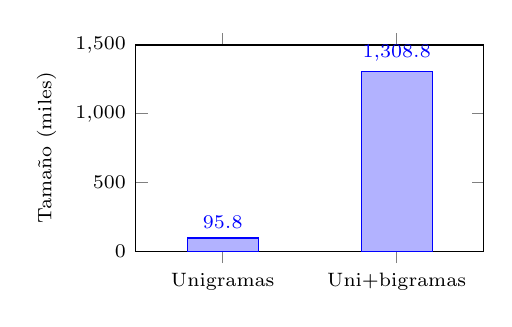
\begin{tikzpicture}
					\begin{axis}[
							ybar, width=6cm, height=4.2cm,
							symbolic x coords={Unigramas, Uni+bigramas},
							xtick=data, ymin=0, ymax=1500,
							ylabel={\scriptsize Tama\~no (miles)},
							nodes near coords, nodes near coords style={font=\scriptsize},
							every axis plot/.append style={fill=UCMBlue!60, draw=UCMNavy},
							tick label style={font=\scriptsize}, bar width=0.9cm,
							enlarge x limits=0.5
						]
						\addplot coordinates {(Unigramas,95.8) (Uni+bigramas,1308.8)};
					\end{axis}
				\end{tikzpicture}

				\small
				De 95\,810 a 1\,308\,842 entradas ($\times 13.7$).
			\end{alertblock}

			\small
			Soluciones: subir \texttt{min\_freq} o reducir la dimensi\'on con \textbf{embeddings}.
		\end{column}
	\end{columns}

\end{frame}

\begin{frame}{TF-IDF}

	\begin{columns}[T]
		\begin{column}{0.53\textwidth}
			En BoW todas las palabras pesan igual, pero ``el'', ``de'', ``a'' aportan poco para clasificar.

			\formula{\centering $w_{ij} = \mathrm{tf}_{ij} \times \log\dfrac{N}{\mathrm{df}_i}$}

			\small
			\begin{itemize}
				\item $\mathrm{tf}_{ij}$: veces que la palabra $i$ aparece en el documento $j$ (el valor BoW).
				\item $N$: n\'umero de documentos de la colecci\'on.
				\item $\mathrm{df}_i$: n\'umero de documentos que contienen la palabra $i$.
			\end{itemize}

			Si una palabra aparece en \emph{todos} los documentos, $\mathrm{df}_i = N$ y $w_{ij} = 0$: se ignora.
		\end{column}

		\begin{column}{0.44\textwidth}
			\begin{block}{En scikit-learn}
				\scriptsize
				\texttt{TfidfVectorizer(ngram\_range=(1,2))}
				\begin{itemize}
					\item IDF suavizado: $\log\frac{1+N}{1+\mathrm{df}_i} + 1$.
					\item Cada vector se normaliza a norma $L_2$ unitaria.
				\end{itemize}
				`My dog likes hot dogs on a hot day.' $\to$ ``hot'' recibe $0.66$; ``dog'', ``dogs'', ``hot dogs'' reciben $0.43$.
			\end{block}

			\begin{alertblock}{L\'imite de las representaciones por conteo}
				\small
				No representan \textbf{significado} ni \textbf{orden}.
				\begin{quote}
					\scriptsize\itshape ``The complete meaning of a word is always contextual, and no study of meaning apart from context can be taken seriously.'' --- J.\,R.\ Firth, 1935
				\end{quote}
			\end{alertblock}
		\end{column}
	\end{columns}

\end{frame}

% =================================================================
\section{Embeddings de Palabras}

\begin{frame}{Hip\'otesis Distribucional}

	\begin{columns}[c]
		\begin{column}{0.5\textwidth}
			\begin{block}{Idea}
				``Conocer\'as una palabra por la compa\~n\'ia que mantiene'' (Firth, 1957).\\[3pt]
				Palabras que aparecen en contextos parecidos tienen significados parecidos.
			\end{block}

			\begin{itemize}
				\small
				\item ``Tom\'e un \underline{\hspace{1cm}} de caf\'e'': taza, vaso, sorbo.
				\item Un \textbf{embedding} asigna a cada palabra un vector denso $\mathbf{v}_w \in \R^d$ con $d \ll |\V|$.
				\item Se aprende \textbf{prediciendo el contexto}: autosupervisado.
			\end{itemize}
		\end{column}

		\begin{column}{0.47\textwidth}
			\centering
			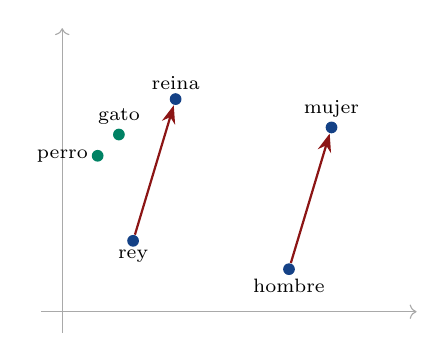
\begin{tikzpicture}[scale=0.9,
					pt/.style={circle, fill=UCMNavy, inner sep=1.5pt},
					lb/.style={font=\scriptsize}
				]
				\draw[->, mitgray] (-0.3,0) -- (5,0);
				\draw[->, mitgray] (0,-0.3) -- (0,4);
				\node[pt] (r) at (1,1) {}; \node[lb, below] at (r) {rey};
				\node[pt] (q) at (1.6,3) {}; \node[lb, above] at (q) {reina};
				\node[pt] (h) at (3.2,0.6) {}; \node[lb, below] at (h) {hombre};
				\node[pt] (m) at (3.8,2.6) {}; \node[lb, above] at (m) {mujer};
				\draw[-{Stealth}, StanfordRed, thick] (r) -- (q);
				\draw[-{Stealth}, StanfordRed, thick] (h) -- (m);
				\node[pt, fill=AccentGreen] at (0.5,2.2) {}; \node[lb, left] at (0.5,2.2) {perro};
				\node[pt, fill=AccentGreen] at (0.8,2.5) {}; \node[lb, above] at (0.8,2.5) {gato};
			\end{tikzpicture}

			\small
			Direcciones del espacio codifican relaciones: $\mathbf{v}_{\text{reina}} - \mathbf{v}_{\text{rey}} \approx \mathbf{v}_{\text{mujer}} - \mathbf{v}_{\text{hombre}}$.
		\end{column}
	\end{columns}

\end{frame}

\begin{frame}[shrink]{word2vec: Skip-gram y CBOW}

	\begin{columns}[T]
		\begin{column}{0.5\textwidth}
			\centering
			\textbf{\small Skip-gram}: la central predice el contexto\\[4pt]
			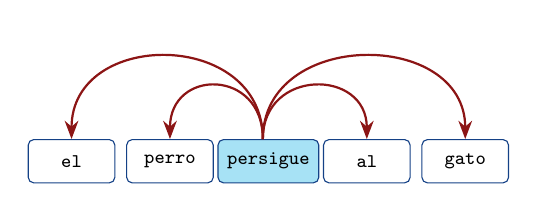
\begin{tikzpicture}[
					w/.style={draw=UCMNavy, rounded corners=2pt, minimum height=0.55cm, minimum width=1.1cm, font=\scriptsize\ttfamily, fill=white},
					c/.style={w, fill=UCMBlue!35, font=\scriptsize\bfseries\ttfamily}
				]
				\node[w] (a1) at (0,0) {el};
				\node[w] (a2) at (1.25,0) {perro};
				\node[c] (a3) at (2.5,0) {persigue};
				\node[w] (a4) at (3.75,0) {al};
				\node[w] (a5) at (5,0) {gato};
				\foreach \n/\h in {a1/1.4,a2/0.9,a4/0.9,a5/1.4}{\draw[-{Stealth}, StanfordRed, thick] ([xshift=-2pt]a3.north) .. controls +(0,\h) and +(0,\h) .. (\n.north);}
			\end{tikzpicture}
			\vspace{0.2cm}
			\formula{\small $P(w_o \mid w_c) = \dfrac{\exp(\mathbf{u}_o^\top \mathbf{v}_c)}{\sum_{i\in\V} \exp(\mathbf{u}_i^\top \mathbf{v}_c)}$}
			\raggedright\scriptsize
			Cada palabra tiene dos vectores: $\mathbf{v}_i$ como \emph{central} y $\mathbf{u}_i$ como \emph{contexto}.
		\end{column}

		\begin{column}{0.5\textwidth}
			\centering
			\textbf{\small CBOW}: el contexto predice la central\\[4pt]
			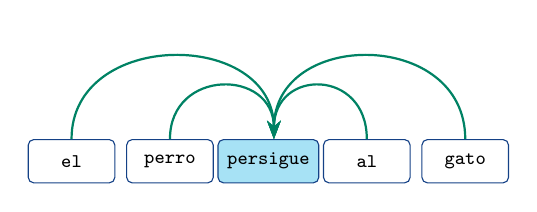
\begin{tikzpicture}[
					w/.style={draw=UCMNavy, rounded corners=2pt, minimum height=0.55cm, minimum width=1.1cm, font=\scriptsize\ttfamily, fill=white},
					c/.style={w, fill=UCMBlue!35, font=\scriptsize\bfseries\ttfamily}
				]
				\node[w] (a1) at (0,0) {el};
				\node[w] (a2) at (1.25,0) {perro};
				\node[c] (a3) at (2.5,0) {persigue};
				\node[w] (a4) at (3.75,0) {al};
				\node[w] (a5) at (5,0) {gato};
				\foreach \n/\h in {a1/1.4,a2/0.9,a4/0.9,a5/1.4}{\draw[-{Stealth}, AccentGreen, thick] (\n.north) .. controls +(0,\h) and +(0,\h) .. ([xshift=2pt]a3.north);}
			\end{tikzpicture}
			\vspace{0.2cm}
			\formula{\small $P(w_c \mid \mathcal{W}_o) = \dfrac{\exp(\mathbf{u}_c^\top \bar{\mathbf{v}}_o)}{\sum_{i\in\V} \exp(\mathbf{u}_i^\top \bar{\mathbf{v}}_o)}$}
			\raggedright\scriptsize
			Promedia los $2m$ vectores de contexto (ventana $m$): $\bar{\mathbf{v}}_o = \frac{1}{2m}\sum_{k=1}^{2m}\mathbf{v}_{o_k}$.
		\end{column}
	\end{columns}

	\vspace{0.2cm}

	\begin{block}{Verosimilitud de skip-gram (texto de largo $T$, ventana $m$)}
		\centering
		$\displaystyle \prod_{t=1}^{T} \prod_{\substack{-m\le j\le m\\ j\ne 0}} P\big(w^{(t+j)} \mid w^{(t)}\big)
			\quad\Longrightarrow\quad
			\mathcal{L} = -\sum_{t=1}^{T} \sum_{\substack{-m\le j\le m\\ j\ne 0}} \log P\big(w^{(t+j)} \mid w^{(t)}\big)$
	\end{block}

\end{frame}

\begin{frame}{Gradiente de Skip-gram y su Costo}

	\begin{columns}[T]
		\begin{column}{0.53\textwidth}
			Tomando logaritmo:
			\[
				\log P(w_o\mid w_c) = \mathbf{u}_o^\top \mathbf{v}_c - \log\Big(\sum_{i\in\V}\exp(\mathbf{u}_i^\top \mathbf{v}_c)\Big)
			\]
			\formula{\centering $\dfrac{\partial \log P(w_o\mid w_c)}{\partial \mathbf{v}_c} = \mathbf{u}_o - \displaystyle\sum_{j\in\V} P(w_j \mid w_c)\,\mathbf{u}_j$}
			\small
			Vector del contexto \textbf{observado} menos el vector de contexto \textbf{esperado} bajo el modelo.
		\end{column}

		\begin{column}{0.44\textwidth}
			\begin{alertblock}{Problema}
				\small
				Cada paso de SGD requiere $P(w_j\mid w_c)$ para \textbf{todo} $j\in\V$: costo $O(|\V|)$, con $|\V|$ de cientos de miles o millones.
			\end{alertblock}

			\begin{block}{Dos aproximaciones}
				\small
				\begin{itemize}
					\item \textbf{Muestreo negativo}: clasificaci\'on binaria contra $K$ palabras de ruido. Costo $O(K)$.
					\item \textbf{Softmax jer\'arquico}: \'arbol binario sobre el vocabulario. Costo $O(\log_2 |\V|)$.
				\end{itemize}
			\end{block}

			{\scriptsize Tras entrenar, skip-gram usa $\mathbf{v}_i$ como embedding; CBOW usa los vectores de contexto.}
		\end{column}
	\end{columns}

\end{frame}

\begin{frame}{Muestreo Negativo}

	\begin{columns}[T]
		\begin{column}{0.52\textwidth}
			\small
			Modelar si $(w_c, w_o)$ es un par real del corpus ($D=1$):
			\[
				P(D=1 \mid w_c, w_o) = \sigma(\mathbf{u}_o^\top \mathbf{v}_c), \qquad \sigma(x) = \frac{1}{1+e^{-x}}
			\]
			S\'olo con pares positivos la soluci\'on trivial es hacer los vectores enormes ($\sigma \to 1$). Se a\~naden $K$ palabras de \textbf{ruido} $w_k \sim P(w)$:
			\begin{center}
				\resizebox{\linewidth}{!}{$\displaystyle P(w^{(t+j)}\mid w^{(t)}) \approx P(D=1\mid w^{(t)}, w^{(t+j)}) \prod_{k=1}^{K} P(D=0\mid w^{(t)}, w_k)$}
			\end{center}
		\end{column}

		\begin{column}{0.45\textwidth}
			\formula{\small $-\log \sigma\big(\mathbf{u}_{i_{t+j}}^\top \mathbf{v}_{i_t}\big) - \displaystyle\sum_{k=1}^{K} \log \sigma\big(-\mathbf{u}_{h_k}^\top \mathbf{v}_{i_t}\big)$}
			\scriptsize
			$i_t$: \'indice central; $i_{t+j}$: contexto real; $h_k$: ruido.

			\vspace{0.2cm}

			\begin{block}{Distribuci\'on de ruido}
				\small
				\[
					P(w) \propto \mathrm{count}(w)^{0.75}
				\]
				Suaviza la frecuencia: las palabras raras se muestrean m\'as que en proporci\'on a su frecuencia. En d2l, $K=5$.
			\end{block}

			\small
			Es una \textbf{entrop\'ia cruzada binaria}: 1 para el contexto real, 0 para el ruido.
		\end{column}
	\end{columns}

\end{frame}

\begin{frame}{Softmax Jer\'arquico}

	\begin{columns}[c]
		\begin{column}{0.45\textwidth}
			\centering
			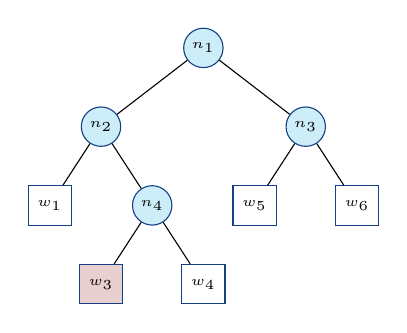
\begin{tikzpicture}[
					level distance=1cm,
					level 1/.style={sibling distance=2.6cm},
					level 2/.style={sibling distance=1.3cm},
					inn/.style={circle, draw=UCMNavy, fill=UCMBlue!20, minimum size=5mm, inner sep=0pt, font=\tiny},
					leaf/.style={rectangle, draw=UCMNavy, fill=white, minimum size=5mm, font=\tiny}
				]
				\node[inn] {$n_1$}
				child {node[inn] {$n_2$}
						child {node[leaf] {$w_1$}}
						child {node[inn] {$n_4$}
								child {node[leaf, fill=StanfordRed!20] {$w_3$}}
								child {node[leaf] {$w_4$}}
							}
					}
				child {node[inn] {$n_3$}
						child {node[leaf] {$w_5$}}
						child {node[leaf] {$w_6$}}
					};
			\end{tikzpicture}

			\scriptsize
			Camino a $w_3$: izquierda, derecha, izquierda.
		\end{column}

		\begin{column}{0.52\textwidth}
			\small
			Las palabras son hojas; cada nodo interno $n$ tiene un vector $\mathbf{u}_n$. En cada nodo se decide izquierda/derecha con una sigmoide:
			\formula{\small $P(w_o\mid w_c) = \displaystyle\prod_{j=1}^{L(w_o)-1} \sigma\Big(\big[\!\big[ n(w_o,j{+}1) = \mathrm{izq}(n(w_o,j)) \big]\!\big]\, \mathbf{u}_{n(w_o,j)}^\top \mathbf{v}_c\Big)$}
			\scriptsize
			$[\![x]\!] = +1$ si $x$ es verdadero y $-1$ si no; $L(w)$: nodos en el camino de la ra\'iz a $w$.
			\small
			\[
				P(w_3\mid w_c) = \sigma(\mathbf{u}_{n_1}^\top\mathbf{v}_c)\,\sigma(-\mathbf{u}_{n_2}^\top\mathbf{v}_c)\,\sigma(\mathbf{u}_{n_4}^\top\mathbf{v}_c)
			\]
			Como $\sigma(x)+\sigma(-x)=1$, las probabilidades suman 1 sin normalizar. Costo $O(\log_2|\V|)$.
		\end{column}
	\end{columns}

\end{frame}

\begin{frame}{Preparar los Datos para word2vec (PTB)}

	\begin{columns}[T]
		\begin{column}{0.5\textwidth}
			\begin{block}{1. Vocabulario}
				\small
				42\,069 oraciones; \texttt{min\_freq=10} $\Rightarrow$ $|\V| = 6\,719$. El resto $\to$ \tok{<unk>}.
			\end{block}

			\begin{block}{2. Submuestreo de palabras frecuentes}
				\small
				Cada token $w_i$ se descarta con probabilidad
				\formula{\centering $P(w_i) = \max\Big(1 - \sqrt{\dfrac{t}{f(w_i)}},\ 0\Big),\quad t = 10^{-4}$}
				$f(w_i)$: frecuencia relativa. ``the'': de 50\,770 a $\sim$2\,010 apariciones; ``join'' conserva sus 45.
			\end{block}
		\end{column}

		\begin{column}{0.47\textwidth}
			\begin{block}{3. Pares central--contexto}
				\small
				Para cada palabra central se sortea una ventana entre 1 y \texttt{max\_window\_size}$=5$. Resultado: $\sim$1.5\,M pares.
			\end{block}

			\begin{block}{4. Negativos y minilotes}
				\small
				$K=5$ ruidos por cada palabra de contexto. Como cada central tiene un n\'umero distinto de contextos, se rellena con ceros y se usa una \textbf{m\'ascara}:
				\begin{center}
					\scriptsize
					\begin{tabular}{@{}lc@{}}
						\toprule
						Campo & Forma (lote 512) \\
						\midrule
						\texttt{centers} & $(512, 1)$ \\
						\texttt{contexts\_negatives} & $(512, 60)$ \\
						\texttt{masks}, \texttt{labels} & $(512, 60)$ \\
						\bottomrule
					\end{tabular}
				\end{center}
			\end{block}
		\end{column}
	\end{columns}

\end{frame}

\begin{frame}[fragile]{Entrenar Skip-gram con Muestreo Negativo}

	\begin{columns}[T]
		\begin{column}{0.55\textwidth}
			\begin{tcolorbox}[codebox]
\scriptsize
\begin{verbatim}
embed_size = 100
net = nn.Sequential(
    nn.Embedding(len(vocab), embed_size),  # v
    nn.Embedding(len(vocab), embed_size))  # u

def skip_gram(center, ctx_neg, embed_v, embed_u):
    v = embed_v(center)        # (B, 1, d)
    u = embed_u(ctx_neg)       # (B, L, d)
    return torch.bmm(v, u.permute(0, 2, 1))  # (B,1,L)

# perdida: BCE con logits, enmascarada
l = F.binary_cross_entropy_with_logits(
        pred.reshape(label.shape), label,
        weight=mask, reduction='none').mean(1)
l = l / mask.sum(1) * mask.shape[1]
\end{verbatim}
			\end{tcolorbox}
			\scriptsize Adam, $\eta=0.002$, 5 \'epocas, lote 512. P\'erdida final $\approx 0.41$.
		\end{column}

		\begin{column}{0.42\textwidth}
			\begin{block}{Uso: vecinos m\'as cercanos}
				\small
				Similitud coseno entre $\mathbf{v}_{\text{query}}$ y todas las filas de la matriz de embeddings.\\[3pt]
				Consulta ``chip'' (PTB, $d=100$):
				\begin{center}
					\begin{tabular}{@{}lc@{}}
						\toprule
						Vecino & coseno \\
						\midrule
						microprocessor & 0.70 \\
						mips & 0.65 \\
						intel & 0.64 \\
						\bottomrule
					\end{tabular}
				\end{center}
			\end{block}

			{\small Nadie le dijo al modelo que ``chip'' es un componente electr\'onico: lo dedujo de los contextos.}
		\end{column}
	\end{columns}

\end{frame}

\begin{frame}{GloVe: Estad\'isticas Globales de Co-ocurrencia}

	\begin{columns}[T]
		\begin{column}{0.52\textwidth}
			\small
			Sea $x_{ij}$ el n\'umero de veces que $w_j$ aparece en el contexto de $w_i$ en \emph{todo} el corpus. Skip-gram puede reescribirse como
			\[
				-\sum_{i\in\V}\sum_{j\in\V} x_{ij}\log q_{ij}, \qquad q_{ij} = \frac{\exp(\mathbf{u}_j^\top\mathbf{v}_i)}{\sum_{k}\exp(\mathbf{u}_k^\top\mathbf{v}_i)}
			\]
			Problemas: normalizar $q_{ij}$ es caro, y las co-ocurrencias raras pesan demasiado. GloVe usa una \textbf{p\'erdida cuadr\'atica en log-conteos}:
			\formula{\small $\displaystyle\sum_{i\in\V}\sum_{j\in\V} h(x_{ij})\big(\mathbf{u}_j^\top\mathbf{v}_i + b_i + c_j - \log x_{ij}\big)^2$}
			\scriptsize
			$h(x) = (x/c)^{\alpha}$ si $x<c$, si no $1$; con $\alpha=0.75$, $c=100$. Como $h(0)=0$, s\'olo se muestrean pares con $x_{ij}>0$. Por simetr\'ia, el embedding final es $\mathbf{u}_i + \mathbf{v}_i$.
		\end{column}

		\begin{column}{0.45\textwidth}
			\begin{block}{¿Por qu\'e funciona? Cocientes}
				\scriptsize
				\setlength{\tabcolsep}{3pt}
				\begin{tabular}{@{}lcccc@{}}
					\toprule
					$w_k$ & solid & gas & water & fashion \\
					\midrule
					$P(w_k\mid\text{ice})$ & 0.00019 & 0.000066 & 0.003 & 0.000017 \\
					$P(w_k\mid\text{steam})$ & 0.000022 & 0.00078 & 0.0022 & 0.000018 \\
					\midrule
					cociente & \textbf{8.9} & \textbf{0.085} & 1.36 & 0.96 \\
					\bottomrule
				\end{tabular}
				\\[4pt]
				\small
				El \textbf{cociente} separa lo que distingue a hielo de vapor (s\'olido vs.\ gas) de lo que comparten (agua) o no les concierne (moda). GloVe ajusta
				$(\mathbf{u}_j-\mathbf{u}_k)^\top\mathbf{v}_i \approx \log(p_{ij}/p_{ik})$.
			\end{block}
			{\tiny Pennington, Socher \& Manning (2014), Tabla 1.}
		\end{column}
	\end{columns}

\end{frame}

\begin{frame}{Embeddings de Subpalabras: fastText}

	\begin{columns}[T]
		\begin{column}{0.5\textwidth}
			\begin{block}{Motivaci\'on}
				\small
				word2vec y GloVe tratan ``perro'', ``perros'', ``perrito'' como s\'imbolos independientes y no tienen vector para palabras \textbf{fuera del vocabulario}. En espa\~nol, con su rica morfolog\'ia (``comer, comemos, comi\'eramos\ldots''), el problema es grave.
			\end{block}

			\formula{\centering $\mathbf{v}_w = \displaystyle\sum_{g\in\mathcal{G}_w} \mathbf{z}_g$}
			\small
			$\mathcal{G}_w$: $n$-gramas de caracteres de largo 3 a 6 de la palabra m\'as la palabra completa; $\mathbf{z}_g$: vector del subtoken $g$. El resto es skip-gram.
		\end{column}

		\begin{column}{0.47\textwidth}
			\begin{block}{Ejemplo: ``where'' con $n=3$}
				\centering
				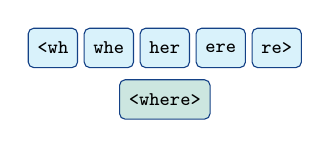
\begin{tikzpicture}[g/.style={draw=UCMNavy, fill=UCMBlue!15, rounded corners=2pt, font=\scriptsize\ttfamily, minimum height=0.5cm}]
					\node[g] (a) at (0,0) {<wh};
					\node[g, right=2pt of a] (b) {whe};
					\node[g, right=2pt of b] (c) {her};
					\node[g, right=2pt of c] (d) {ere};
					\node[g, right=2pt of d] (e) {re>};
					\node[g, fill=AccentGreen!20, below=4pt of c] {<where>};
				\end{tikzpicture}

				\vspace{2pt}
				\scriptsize Los s\'imbolos \texttt{<} y \texttt{>} marcan inicio y fin de palabra: \texttt{<her>} (``her'') $\neq$ \texttt{her} (dentro de ``where'').
			\end{block}

			\begin{itemize}
				\small
				\item \good\ Palabras raras y nuevas obtienen buenos vectores por subpalabras compartidas.
				\item \bad\ M\'as par\'ametros: el vocabulario de subtokens es mucho mayor.
			\end{itemize}
		\end{column}
	\end{columns}

\end{frame}

\begin{frame}{Byte Pair Encoding (BPE)}

	\begin{columns}[T]
		\begin{column}{0.48\textwidth}
			\begin{block}{Algoritmo}
				\small
				\begin{enumerate}
					\item Inicializar los s\'imbolos con los caracteres, el fin de palabra \texttt{\_} y \texttt{[UNK]}.
					\item Escribir cada palabra como secuencia de s\'imbolos con su frecuencia.
					\item Contar los pares adyacentes (ponderados por frecuencia) y \textbf{fusionar el m\'as frecuente} en un s\'imbolo nuevo.
					\item Repetir el paso 3 un n\'umero fijo de veces.
				\end{enumerate}
			\end{block}
			\small
			Produce subpalabras de \textbf{largo variable} con un vocabulario de \textbf{tama\~no fijo}. Lo usan GPT y la mayor\'ia de los LLMs actuales.
		\end{column}

		\begin{column}{0.49\textwidth}
			\begin{block}{Ejemplo (d2l)}
				\scriptsize
				Corpus: \texttt{fast\_}$\times 4$, \texttt{faster\_}$\times 3$, \texttt{tall\_}$\times 5$, \texttt{taller\_}$\times 4$.\\[3pt]
				\setlength{\tabcolsep}{4pt}
				\begin{tabular}{@{}cl@{\hspace{10pt}}cl@{}}
					\toprule
					\# & fusi\'on & \# & fusi\'on \\
					\midrule
					1 & \texttt{t a} $\to$ \texttt{ta} & 6 & \texttt{fas t} $\to$ \texttt{fast} \\
					2 & \texttt{ta l} $\to$ \texttt{tal} & 7 & \texttt{e r} $\to$ \texttt{er} \\
					3 & \texttt{tal l} $\to$ \texttt{tall} & 8 & \texttt{er \_} $\to$ \texttt{er\_} \\
					4 & \texttt{f a} $\to$ \texttt{fa} & 9 & \texttt{tall \_} $\to$ \texttt{tall\_} \\
					5 & \texttt{fa s} $\to$ \texttt{fas} & 10 & \texttt{fast \_} $\to$ \texttt{fast\_} \\
					\bottomrule
				\end{tabular}
				\\[4pt]
				Segmentaci\'on de palabras nuevas (prefijo m\'as largo):\\
				\texttt{tallest\_} $\to$ \texttt{tall e s t \_}\\
				\texttt{fatter\_} $\to$ \texttt{fa t t er\_}
			\end{block}
		\end{column}
	\end{columns}

\end{frame}

\begin{frame}{Similitud y Analog\'ias con GloVe Preentrenado}

	\begin{columns}[T]
		\begin{column}{0.48\textwidth}
			\begin{block}{Vecinos m\'as cercanos (GloVe 6B, $d=50$)}
				\scriptsize
				\begin{tabular}{@{}lll@{}}
					\toprule
					Consulta & \multicolumn{2}{l}{Vecinos (coseno)} \\
					\midrule
					chip & chips (0.86) & intel (0.75) \\
					baby & babies (0.84) & boy (0.80) \\
					beautiful & lovely (0.92) & gorgeous (0.89) \\
					\bottomrule
				\end{tabular}
				\\[3pt]
				400\,000 palabras, entrenado sobre Wikipedia.
			\end{block}

			\small
			\begin{itemize}
				\item Comparado con el word2vec de PTB, un corpus m\'as grande da vecinos m\'as limpios.
				\item Se usan sin reentrenar: es la forma m\'as simple de \textbf{transferencia} en NLP.
			\end{itemize}
		\end{column}

		\begin{column}{0.49\textwidth}
			\begin{block}{Analog\'ias $a : b :: c : d$}
				\formula{\centering $d = \arg\max_{w}\ \cos\big(\mathbf{v}_w,\ \mathbf{v}_c + \mathbf{v}_b - \mathbf{v}_a\big)$}
				\scriptsize
				\begin{tabular}{@{}ll@{}}
					\toprule
					Analog\'ia & Tipo \\
					\midrule
					man : woman :: son : \textbf{daughter} & sem\'antica \\
					beijing : china :: tokyo : \textbf{japan} & sem\'antica \\
					bad : worst :: big : \textbf{biggest} & sint\'actica \\
					do : did :: go : \textbf{went} & sint\'actica \\
					\bottomrule
				\end{tabular}
			\end{block}

			\begin{alertblock}{Cuidado}
				\small
				Las mismas operaciones revelan \textbf{sesgos} del corpus (p.\ ej.\ g\'enero y profesiones).
			\end{alertblock}
		\end{column}
	\end{columns}

\end{frame}

% =================================================================
\section{Representaciones Contextuales}

\begin{frame}{De Embeddings Est\'aticos a Contextuales}

	\begin{columns}[T]
		\begin{column}{0.5\textwidth}
			\begin{alertblock}{Limitaci\'on de word2vec y GloVe}
				\small
				Una palabra $\Rightarrow$ un vector $f(x)$, sin importar el contexto:
				\begin{itemize}
					\item ``fui al \textbf{banco} a depositar dinero''
					\item ``me sent\'e en el \textbf{banco} de la plaza''
				\end{itemize}
				reciben el mismo $\mathbf{v}_{\text{banco}}$.
			\end{alertblock}

			\begin{block}{Representaci\'on sensible al contexto}
				\small
				$f(x, c(x))$: el vector de un token depende de la oraci\'on completa. Ejemplos: TagLM, CoVe, \textbf{ELMo}.
			\end{block}
		\end{column}

		\begin{column}{0.47\textwidth}
			\begin{block}{Comparaci\'on}
				\scriptsize
				\setlength{\tabcolsep}{3pt}
				\begin{tabular}{@{}l>{\raggedright}p{1.5cm}>{\raggedright}p{1.5cm}>{\raggedright\arraybackslash}p{1.65cm}@{}}
					\toprule
					& \textbf{ELMo} & \textbf{GPT} & \textbf{BERT} \\
					\midrule
					Contexto & bidireccional & izq.\ $\to$ der. & bidireccional \\
					Red & biLSTM & Transformer decoder & Transformer encoder \\
					Tarea final & arquitectura espec\'ifica & gen\'erica & gen\'erica \\
					Ajuste & red congelada, se a\~naden rasgos & todos los par\'ametros & todos los par\'ametros + capa de salida \\
					\bottomrule
				\end{tabular}
			\end{block}

			\small
			BERT combina lo mejor de ambos: contexto \textbf{bidireccional} (ELMo) y arquitectura \textbf{agn\'ostica a la tarea} (GPT).
		\end{column}
	\end{columns}

\end{frame}

\begin{frame}{BERT: Representaci\'on de la Entrada}

	\centering
	\resizebox{\textwidth}{!}{%
	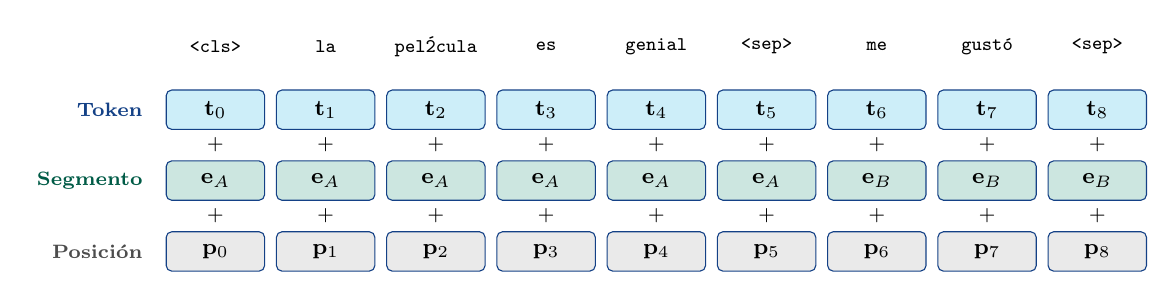
\begin{tikzpicture}[
			t/.style={draw=UCMNavy, rounded corners=2pt, minimum width=1.25cm, minimum height=0.5cm, font=\tiny\ttfamily, fill=white, inner sep=1pt},
			tk/.style={t, fill=UCMBlue!20},
			sg/.style={t, fill=AccentGreen!20},
			ps/.style={t, fill=mitgray!25}
		]
		\foreach \w [count=\i from 0] in {<cls>,la,pel\'icula,es,genial,<sep>,me,gust\'o,<sep>}{
			\node[font=\scriptsize\ttfamily] (in\i) at (\i*1.4, 2.0) {\w};
			\node[tk] (tk\i) at (\i*1.4, 1.2) {\footnotesize $\mathbf{t}_{\i}$};
			\node at (\i*1.4, 0.75) {\scriptsize $+$};
			\node at (\i*1.4, -0.15) {\scriptsize $+$};
			\node[ps] (ps\i) at (\i*1.4, -0.6) {\footnotesize $\mathbf{p}_{\i}$};
		}
		\foreach \i in {0,...,5}{\node[sg] at (\i*1.4, 0.3) {\footnotesize $\mathbf{e}_A$};}
		\foreach \i in {6,7,8}{\node[sg] at (\i*1.4, 0.3) {\footnotesize $\mathbf{e}_B$};}
		\node[font=\scriptsize\bfseries, anchor=east, text=UCMNavy] at (-0.8, 1.2) {Token};
		\node[font=\scriptsize\bfseries, anchor=east, text=AccentGreen!70!black] at (-0.8, 0.3) {Segmento};
		\node[font=\scriptsize\bfseries, anchor=east, text=black!70] at (-0.8, -0.6) {Posici\'on};
	\end{tikzpicture}}

	\vspace{0.3cm}

	\begin{columns}[T]
		\begin{column}{0.5\textwidth}
			\formula{\centering $\mathbf{x}_i = \mathbf{e}_{\text{tok}}(t_i) + \mathbf{e}_{\text{seg}}(s_i) + \mathbf{e}_{\text{pos}}(i)$}
			\small
			Los embeddings de posici\'on se \textbf{aprenden} (a diferencia de los sinusoidales del Transformer original).
		\end{column}

		\begin{column}{0.47\textwidth}
			\small
			\begin{itemize}
				\item Un texto: \tok{<cls>} $A$ \tok{<sep>}.
				\item Par de textos: \tok{<cls>} $A$ \tok{<sep>} $B$ \tok{<sep>}.
				\item La salida en \tok{<cls>} resume toda la secuencia: se usa para clasificar.
			\end{itemize}
		\end{column}
	\end{columns}

\end{frame}

\begin{frame}[shrink]{BERT: Tareas de Preentrenamiento}

	\begin{columns}[T]
		\begin{column}{0.5\textwidth}
			\begin{block}{Masked Language Modeling (MLM)}
				\small
				Se elige al azar el \textbf{15\%} de los tokens para predecir. De ellos:
				\begin{center}
					\begin{tabular}{@{}cl@{}}
						\toprule
						80\% & $\to$ \tok{<mask>} \\
						10\% & $\to$ un token aleatorio \\
						10\% & $\to$ se deja igual \\
						\bottomrule
					\end{tabular}
				\end{center}
				\tok{<mask>} nunca aparece al ajustar en la tarea final; los casos aleatorio e intacto reducen ese desajuste. Cabeza: MLP de una capa oculta + entrop\'ia cruzada sobre $\V$.
			\end{block}
		\end{column}

		\begin{column}{0.47\textwidth}
			\begin{block}{Next Sentence Prediction (NSP)}
				\small
				Clasificaci\'on binaria: ¿es $B$ la oraci\'on que sigue a $A$?
				\begin{itemize}
					\item 50\% pares reales, 50\% oraci\'on aleatoria.
					\item Se usa la salida en \tok{<cls>}: capa oculta $\tanh$ + 2 salidas.
				\end{itemize}
			\end{block}

			\formula{\centering $\mathcal{L}_{\text{BERT}} = \mathcal{L}_{\text{MLM}} + \mathcal{L}_{\text{NSP}}$}

			\begin{block}{Escala}
				\scriptsize
				\setlength{\tabcolsep}{3pt}
				\begin{tabular}{@{}lcccc@{}}
					\toprule
					& capas & oculta & cabezas & par\'ametros \\
					\midrule
					BERT\textsubscript{BASE} & 12 & 768 & 12 & 110\,M \\
					BERT\textsubscript{LARGE} & 24 & 1024 & 16 & 340\,M \\
					\bottomrule
				\end{tabular}
				\\[2pt]
				Corpus: BookCorpus + Wikipedia en ingl\'es ($\sim$3\,300 M palabras).
			\end{block}
		\end{column}
	\end{columns}

\end{frame}

\begin{frame}{Datos para Preentrenar BERT (WikiText-2)}

	\begin{columns}[T]
		\begin{column}{0.5\textwidth}
			\small
			El ciclo de vida de los datos, aplicado a BERT:
			\begin{enumerate}
				\item \textbf{Corpus}: WikiText-2 (m\'as del doble que PTB, conserva may\'usculas, puntuaci\'on y n\'umeros).
				\item \textbf{Limpieza}: p\'arrafos $\geq 2$ oraciones, min\'usculas, barajado.
				\item \textbf{Etiquetas autom\'aticas}: pares NSP desde oraciones adyacentes; posiciones MLM al azar (excluyendo \tok{<cls>} y \tok{<sep>}).
				\item \textbf{Vocabulario}: \texttt{min\_freq=5} + \tok{<pad>}, \tok{<mask>}, \tok{<cls>}, \tok{<sep>} $\Rightarrow |\V| = 20\,256$.
				\item \textbf{Relleno}: secuencias a largo 64 con \tok{<pad>}; pesos 0 para predicciones de relleno.
			\end{enumerate}
		\end{column}

		\begin{column}{0.47\textwidth}
			\begin{block}{Un minilote (lote 512, largo 64)}
				\centering
				\scriptsize
				\begin{tabular}{@{}lc@{}}
					\toprule
					Campo & Forma \\
					\midrule
					\texttt{tokens\_X}, \texttt{segments\_X} & $[512, 64]$ \\
					\texttt{valid\_lens\_x} & $[512]$ \\
					\texttt{pred\_positions\_X} & $[512, 10]$ \\
					\texttt{mlm\_weights\_X}, \texttt{mlm\_Y} & $[512, 10]$ \\
					\texttt{nsp\_y} & $[512]$ \\
					\bottomrule
				\end{tabular}
				\\[3pt]
				$10 = \mathrm{round}(64 \times 0.15)$ predicciones MLM por secuencia.
			\end{block}

			\begin{block}{Resultado}
				\small
				Tras preentrenar, ``crane'' recibe vectores \textbf{distintos} en ``a crane is flying'' y ``a crane driver came'': la representaci\'on depende del contexto.
			\end{block}
		\end{column}
	\end{columns}

\end{frame}

% =================================================================
\section{Conclusiones}

\begin{frame}{Conclusiones}

	\begin{itemize}
		\item El NLP moderno sigue el paradigma \textbf{preentrenar (autosupervisado) $\to$ ajustar (supervisado)}.

		\vspace{0.15cm}

		\item El \textbf{ciclo de vida de los datos} (recolecci\'on, limpieza, anotaci\'on, tokenizaci\'on, representaci\'on, evaluaci\'on, monitoreo) determina en gran parte la calidad del modelo.

		\vspace{0.15cm}

		\item \textbf{Representaciones por conteo} (BoW, $n$-gramas, TF-IDF): simples y fuertes para clasificaci\'on, pero dispersas, sin orden ni significado.

		\vspace{0.15cm}

		\item \textbf{Embeddings est\'aticos} (word2vec, GloVe): vectores densos que capturan similitud y analog\'ias; muestreo negativo y softmax jer\'arquico hacen viable el entrenamiento.

		\vspace{0.15cm}

		\item \textbf{Subpalabras} (fastText, BPE): resuelven morfolog\'ia y palabras fuera del vocabulario.

		\vspace{0.15cm}

		\item \textbf{Representaciones contextuales} (BERT): un vector por token \emph{en su contexto}, base de los modelos de lenguaje actuales.
	\end{itemize}

	\vspace{0.2cm}

	\begin{alertblock}{Para el laboratorio 3.1}
		Construir el vocabulario de AG\_NEWS, entrenar un clasificador lineal sobre BoW y comparar con bigramas y TF-IDF. Probar el efecto de reducir \texttt{vocab\_size} y de subir \texttt{min\_freq}.
	\end{alertblock}

\end{frame}

\begin{frame}{Referencias}

	\small
	\begin{itemize}
		\item A.\ Zhang, Z.\ C.\ Lipton, M.\ Li \& A.\ J.\ Smola, \textit{Dive into Deep Learning}, Cambridge University Press, 2023. Cap.\ 15: \textit{Natural Language Processing: Pretraining}. \texttt{d2l.ai}
		\item T.\ Mikolov et al., ``Distributed Representations of Words and Phrases and their Compositionality'', NeurIPS 2013.
		\item J.\ Pennington, R.\ Socher \& C.\ D.\ Manning, ``GloVe: Global Vectors for Word Representation'', EMNLP 2014.
		\item P.\ Bojanowski et al., ``Enriching Word Vectors with Subword Information'', TACL 2017.
		\item R.\ Sennrich, B.\ Haddow \& A.\ Birch, ``Neural Machine Translation of Rare Words with Subword Units'', ACL 2016.
		\item M.\ E.\ Peters et al., ``Deep Contextualized Word Representations'' (ELMo), NAACL 2018.
		\item J.\ Devlin et al., ``BERT: Pre-training of Deep Bidirectional Transformers for Language Understanding'', NAACL 2019.
		\item T.\ Gebru et al., ``Datasheets for Datasets'', \textit{Communications of the ACM}, 2021.
		\item D.\ Jurafsky \& J.\ H.\ Martin, \textit{Speech and Language Processing}, 3.\textsuperscript{a} ed.\ (borrador). Caps.\ 2 (tokenizaci\'on) y 6 (sem\'antica vectorial).
	\end{itemize}

\end{frame}

\end{document}
